\section{}
    \begin{frame}[allowframebreaks]{Clustering to build phonemes}

        \textbf{K-means}

        The number of clusters was selected using a penalized silhouette criterion, which indicated that five clusters provided the best clustering structure.

        \begin{itemize}
            \item Cluster the zeroth derivative (consonants)
            \item Cluster the first derivative (vowels)
        \end{itemize}

    \end{frame}

    \subsection{}
        \begin{frame}[allowframebreaks]{Clustering lidar's \(0^{\mathrm{th}}\) derivative}
    The five clusters were determined by penalized silhouette analysis.


    Any obstacle beyond the 2.5 m range is set to 4.0 m because only the proximity of the walls is important.
    \begin{figure}[H]
        \centering
        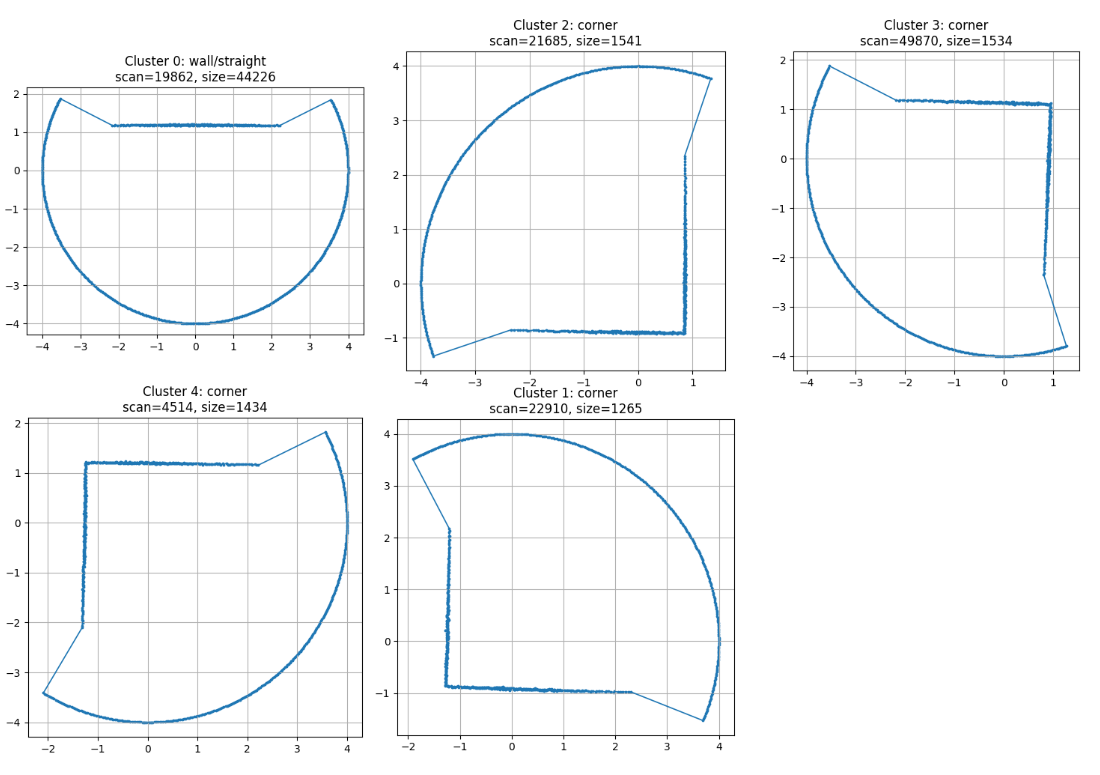
\includegraphics[width=0.9\textwidth]{clustering_lidar_zero_derivative_with_single_sample.png}
    \end{figure}

\end{frame}

        \begin{frame}[allowframebreaks]{Clustering lidar's \(0^{\mathrm{th}}\) derivative}
    The five clusters were determined by penalized silhouette analysis.


    Any obstacle beyond the 2.5 m range is set to 4.0 m because only the proximity of the walls is important.
    \begin{figure}[H]
        \centering
        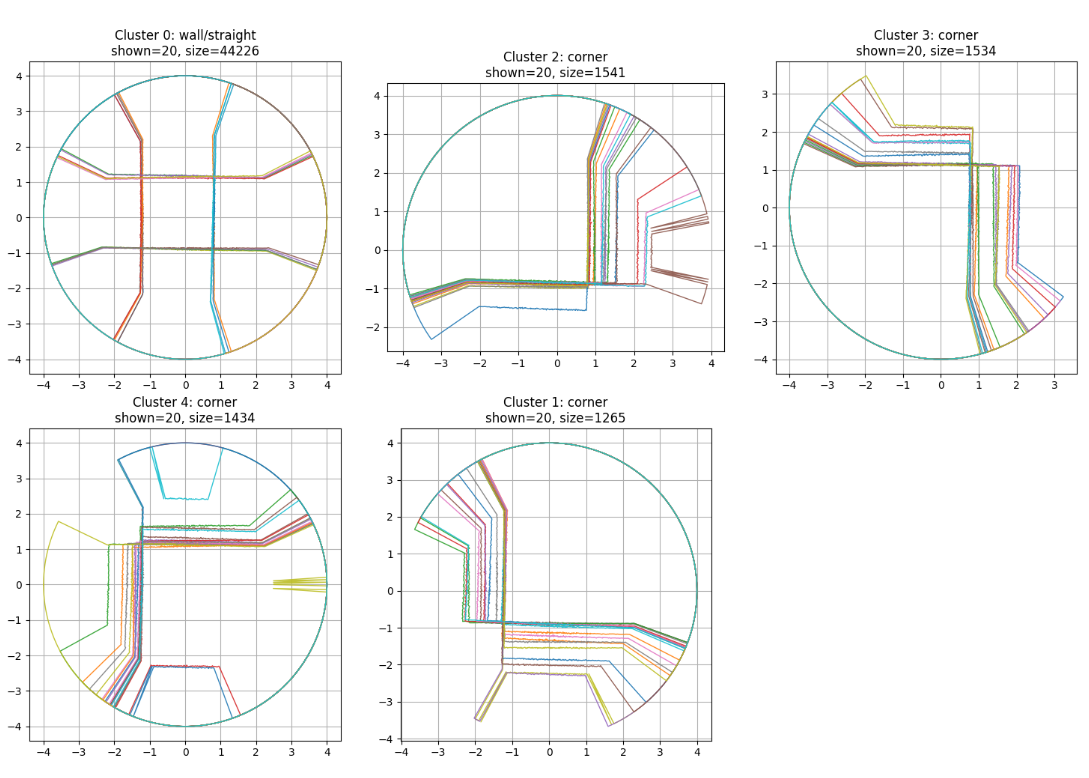
\includegraphics[width=0.9\textwidth]{clustering_lidar_zero_derivative_with_multiple_samples.png}
    \end{figure}

\end{frame}

        \begin{frame}[allowframebreaks]{Clustering LiDAR's \(0^{\mathrm{th}}\) Derivative -- Centroid}
    \begin{itemize}
        \item The centroid will later be used as a new origin for GPS.
        \item The number of clusters is determined by the penalized average silhouette width (ASW) \cite{deng-2024-on-estimation-and-order-selection-for-multivariate-extremes-via-clustering, rousseeuw-1987-silhouettes-a-graphical-aid-to-the-interpretation-and-validation-of-cluster-analysis}
    \end{itemize}

    \begin{algorithm}[H]
    \caption{Penalized ASW Order Selection}
    \begin{algorithmic}[1]
        \State Choose candidate orders \(k \in \{1,\dots,k_{\max}\}\) and small penalty values \(t \in T\).
        \For{each \(k\)}
            \State Cluster the sample \(W\) and obtain centers \(A_k^\ast\) and clusters \(C_1,\dots,C_k\).
            \State Compute \(a(w)\) and \(b(w)\) for each \(w \in W\).
            \State Compute the simplified ASW score \(\bar{s}(k)\).
            \State Compute the penalized score \(S_t(k)\).
        \EndFor
        \State Select \(k^\ast\) from the maximum or turning point of \(S_t(k)\).
    \end{algorithmic}
    \end{algorithm}

    \framebreak

    \begin{figure}
        \centering
        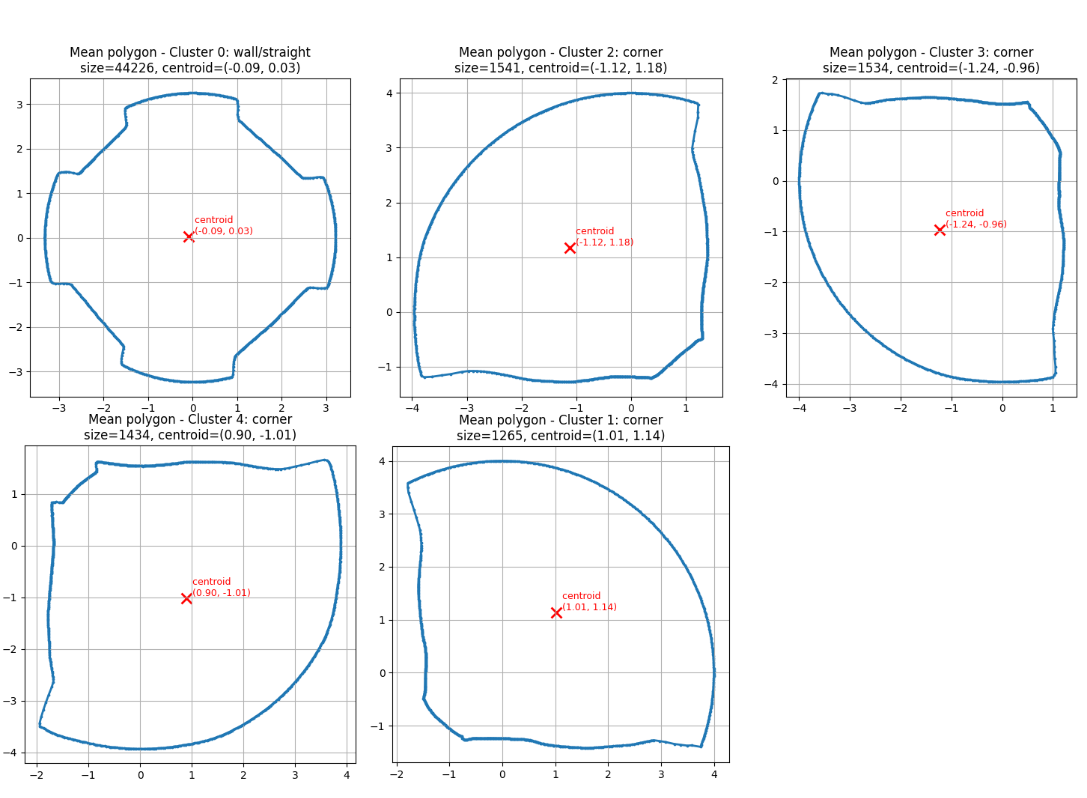
\includegraphics[width=0.9\textwidth]{clustering_lidar_zero_derivative_with_centroid.png}
    \end{figure}
\end{frame}

        \begin{frame}[allowframebreaks]{Phoneme}
    More clusters are formed around the corners.
    \begin{figure}[H]
        \centering
        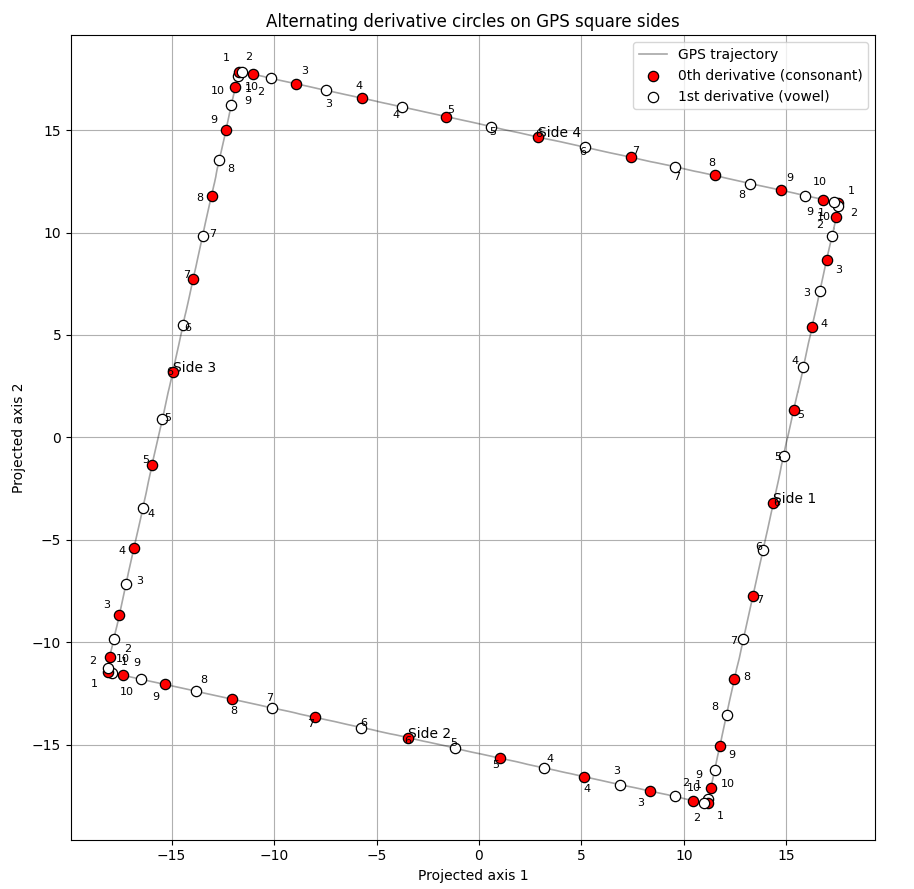
\includegraphics[width=0.7\textwidth]{phonem.png}
    \end{figure}
\end{frame}

